% 最优化方法自学讲义。图示均由 TikZ 绘制，使用 XeLaTeX 连续编译两次。
\documentclass[UTF8,fontset=none,zihao=-4,a4paper]{ctexart}
\usepackage[left=26mm,right=26mm,top=25mm,bottom=25mm,headheight=16pt]{geometry}
\IfFontExistsTF{Songti SC}{
  \setCJKmainfont{Songti SC}[BoldFont={Songti SC Bold}]
  \setCJKsansfont{Songti SC}[BoldFont={Songti SC Bold}]
}{
  \setCJKmainfont{FandolSong-Regular.otf}[BoldFont={FandolSong-Bold.otf}]
  \setCJKsansfont{FandolSong-Regular.otf}[BoldFont={FandolSong-Bold.otf}]
}
\IfFontExistsTF{Times New Roman}{
  \setmainfont{Times New Roman}
}{
  \setmainfont{texgyretermes-regular.otf}[
    BoldFont=texgyretermes-bold.otf,ItalicFont=texgyretermes-italic.otf,
    BoldItalicFont=texgyretermes-bolditalic.otf]
}
\usepackage{amsmath,booktabs,tabularx,array,enumitem,fancyhdr,needspace}
\usepackage{unicode-math}
\setmathfont{texgyretermes-math.otf}
\usepackage{xcolor,tikz}
\usetikzlibrary{arrows.meta,calc}
\usepackage[breakable,skins]{tcolorbox}
\usepackage[hidelinks]{hyperref}
\hypersetup{pdftitle={最优化方法},pdfsubject={运筹学建模与最优化理论基础}}

\definecolor{Theme}{HTML}{35566E}
\definecolor{BoxBack}{HTML}{F2F6F8}
\definecolor{BoxLine}{HTML}{B8C8D3}
\newtcolorbox{infobox}[1]{
  enhanced,breakable,colback=BoxBack,colframe=BoxLine,coltitle=Theme,
  colbacktitle=BoxBack,fonttitle=\normalsize\bfseries,title={#1},
  boxrule=0.5pt,arc=0pt,left=9pt,right=9pt,top=4pt,bottom=4pt,
  toptitle=5pt,bottomtitle=3pt,before skip=5pt,after skip=5pt,parbox=false
}
\tikzset{>=Stealth,every node/.style={font=\small},
  axis/.style={->,thin},curve/.style={Theme,semithick},
  helper/.style={Theme,densely dashed,thin},region/.style={fill=BoxBack}}
\newcounter{worked}[section]
\renewcommand{\theworked}{\thesection.\arabic{worked}}
\newenvironment{worked}[1]{%
  \par\Needspace{6\baselineskip}\refstepcounter{worked}%
  \begin{infobox}{例 \theworked\quad #1}%
}{\end{infobox}}
\newcounter{diagram}[section]
\renewcommand{\thediagram}{\thesection-\arabic{diagram}}
\newcommand{\diagramcaption}[1]{%
  \par\nobreak\smallskip\refstepcounter{diagram}{\small 图 \thediagram\quad #1\par}}
\newcommand{\term}[1]{\textbf{#1}}
\newcommand{\sol}{\par\noindent\textbf{解}\quad}
\newcommand{\ans}[1]{\par\Needspace{3\baselineskip}\noindent\textbf{\ref{#1}}\quad}
\newcommand{\chapterpage}[1]{\clearpage\section{#1}}
\newcommand{\backsection}[1]{%
  \clearpage\phantomsection\section*{#1}\markboth{#1}{}%
  \addcontentsline{toc}{section}{#1}}
\newcommand{\R}{\mathbb{R}}
\newcommand{\transpose}{^{\mathsf T}}
\newcommand{\norm}[1]{\lVert#1\rVert}
\newcommand{\conv}{\operatorname{conv}}
\newcommand{\cone}{\operatorname{cone}}
\newcommand{\rank}{\operatorname{rank}}
\newcommand{\supp}{\operatorname{supp}}
\newcolumntype{Y}{>{\raggedright\arraybackslash}X}

\ctexset{section={format=\large\bfseries,beforeskip=0pt,afterskip=14pt},
  subsection={format=\normalsize\bfseries,beforeskip=12pt,afterskip=6pt},
  subsubsection={format=\normalsize\bfseries,beforeskip=8pt,afterskip=4pt}}
\setcounter{tocdepth}{1}
\setcounter{secnumdepth}{2}
\linespread{1.22}
\setlength{\parindent}{2em}
\setlength{\parskip}{2.5pt}
\setlength{\emergencystretch}{1.5em}
\setlength{\tabcolsep}{6pt}
\renewcommand{\arraystretch}{1.25}
\setlist{itemsep=4pt,topsep=5pt,parsep=0pt,leftmargin=2em}
\clubpenalty=10000
\widowpenalty=10000
\displaywidowpenalty=10000
\allowdisplaybreaks[2]
\raggedbottom
\pagestyle{fancy}
\fancyhf{}
\fancyhead[L]{\small 最优化方法}
\fancyhead[R]{\small\nouppercase{\leftmark}}
\fancyfoot[C]{\small\thepage}
\renewcommand{\headrulewidth}{0.3pt}
\renewcommand{\sectionmark}[1]{\markboth{#1}{}}

\begin{document}
\begin{titlepage}
\thispagestyle{empty}
\vspace*{0.28\textheight}
\begin{center}
{\fontsize{36}{45}\selectfont\bfseries 最优化方法}
\end{center}
\end{titlepage}
\pagenumbering{Roman}
\thispagestyle{empty}
\tableofcontents
\clearpage
\pagenumbering{arabic}

\section{运筹学思想与运筹学建模}\label{sec:model}
生产计划需要决定各产品的产量，设计轻质结构需要决定材料与尺寸。两类问题都要先确定哪些方案可接受，再用同一尺度比较可接受的方案。本章从生产和选址出发建立模型，随后整理第二章所需的向量、投影和微分工具。

\subsection{运筹学处理什么问题}
\term{运筹学}（operations research, OR）运用数学模型和数据为资源配置、组织管理和工程设计提供决策依据。问题中的不确定性、决策者之间的相互作用以及服务流程，分别会引出不同的分析工具。

\begin{center}
\begin{tabularx}{\linewidth}{l Y Y}
\toprule
课件中的方向 & 决策环境 & 代表问题\\
\midrule
分析理论 & 给定数据下比较可行方案，常用数学规划、网络优化 & 已知工时、材料和利润，确定生产数量\\
竞争理论 & 各方收益取决于多方策略，常用博弈论 & 两家企业分别决定是否降价\\
随机服务理论 & 到达或服务时间随机，常用排队论评估等待与利用率 & 在人力成本和等待时间之间选择柜台数\\
\bottomrule
\end{tabularx}
\end{center}

建模时的\term{合伙原则}要求与现场人员共同核对容量、需求和实施条件。\term{催化原则}鼓励检验沿用的工作安排，例如是否可以改变班次。\term{互相渗透原则}要求跨部门核查局部决策的影响，例如增产是否会让仓库超负荷。\term{独立原则}强调对数据和结论独立判断，避免由个别特殊情况概括全局。\term{宽容原则}允许比较多种模型或求解办法。\term{平衡原则}要求把相互牵制的目标和限制放到同一个问题中考虑。

\subsection{从问题描述到模型检验}
\begin{infobox}{方法\quad 建模的工作步骤}
\begin{enumerate}[label=\arabic*.,leftmargin=2em]
\item \term{提出问题}。明确决策范围、评价指标、可控制的量和给定数据。
\item \term{建立模型}。设定变量及其单位，将业务要求写成目标和约束。
\item \term{模型求解}。按模型的结构选用图解、枚举或适用算法。
\item \term{解的检验}。代回约束，核算单位、资源余额及实际可操作性。
\item \term{灵敏性分析}。改变关键参数，比较最优值及推荐方案的变化。
\item \term{解的实施}。把产量、工时、站点等模型输出转换成执行计划。
\item \term{后评估}。用实施结果核对估计值和假设，必要时修订模型。
\end{enumerate}
\end{infobox}

有明确工艺关系时，可以用\term{直接分析法}列出物料或工时平衡。结构与已有问题相近时，可以用\term{类比法}识别变量和约束。复杂流程可以通过\term{模拟法}估计排队或拥堵。\term{数据分析法}从历史记录估计参数，\term{试验分析法}用有计划的试验识别规律。数据和试验都有限时，\term{构想法}可在清楚写出假设的前提下，按不同情景建立方案。

审核模型可问三个问题。模型中的变量和限制能否对应实际对象？用小规模数据能否发现量纲、符号或逻辑错误？能否在保留关键影响的前提下简化求解，例如合并重复限制，或以经检验的线性关系近似单位消耗？

\subsection{决策变量、目标函数和可行集}
\begin{infobox}{定义\quad 数学规划的一般形式}
以列向量 $x=(x_1,\ldots,x_n)\transpose$ 表示决策，以 $f(x)$ 评价方案，以 $S$ 收集满足全部限制的方案。优化问题可写成
\[
  \min_{x\in S} f(x)\qquad\text{或}\qquad \max_{x\in S} f(x).
\]
$S$ 称为\term{可行集}，其中的点称为\term{可行解}。政策或物理限制、变量上下界、非负性和整数性都可用来定义 $S$。
\end{infobox}

设 $p$ 为给定参数，$\xi$ 为随机因素。完整模型中可写 $f(x;p,\xi)$ 及 $g_i(x;p,\xi)$，以区分可选的 $x$、外部给定的 $p$ 和有待描述的 $\xi$。若用固定情景给定 $\xi$，可以得到一个确定性问题。若需在不确定条件下比较方案，还须指定怎样计算收益和判定风险，例如比较不同方案的期望成本。

将下界 $a(x)\ge b$ 写成 $b-a(x)\le 0$，将上界 $a(x)\le b$ 写成 $a(x)-b\le 0$。最大化 $f$ 也可改写成最小化 $-f$，最优决策相同，最优值互为相反数。一个候选点要先通过全部约束，才可与其他方案比较。

\begin{center}
\begin{tabularx}{\linewidth}{l Y}
\toprule
模型类别 & 识别依据及例子\\
\midrule
线性规划 & 连续变量，目标及约束为仿射形式，如按固定单位用量排产\\
非线性规划 & 连续规划中出现真正非线性的目标或约束，如二次能耗成本\\
整数规划 & 部分或全部变量限定为整数，如决定采购台数或站点去留\\
多目标规划 & 同时考虑多个评价指标，如成本与交付时间\\
动态规划 & 问题可按阶段、状态及决策分解，如按月确定库存\\
随机规划 & 参数含随机性，模型明确描述情景、概率及相关决策要求\\
\bottomrule
\end{tabularx}
\end{center}
这些类别可以重叠。按整数台数采购、且需求有多个随机情景的问题，可以同时具有整数和随机结构。线性规划中的“线性”通常允许常数项，因此 $a\transpose x+b$ 也在这一用法内。

\Needspace{8\baselineskip}
\subsection{钢厂生产计划}
\begin{worked}{把生产要求写成线性约束}
计划期内生产 $n$ 种产品。给定各产品的吨利润、设备耗时、原料用量、耗电量、两项生产指标和销售区间，建立利润最大化模型。一般结构对应第 1 章课件的钢厂案例。
\end{worked}
\sol
设 $x_i$ 为第 $i$ 种产品纳入销售计划的产出吨数，$r_i$ 为每吨利润。设 $a_{ij}$、$c_{ij}$ 分别是每吨第 $i$ 种产品占用第 $j$ 类设备的工时和第 $j$ 类材料的数量，$d_i$ 为每吨耗电量。设备可用工时、原料总量和可供电量分别记为 $A_j$、$C_j$ 和 $D$。

先看一项比率指标。令 $b_{ij}>0$ 表示第 $i$ 种产品对第 $j$ 项指标的产出投入比。沿课件的计量口径，产出 $x_i$ 需对应投入 $x_i/b_{ij}$。总产出为正时，总比率至少为 $B_j>0$ 的要求可写成
\[
\frac{\sum_{i=1}^{n}x_i}{\sum_{i=1}^{n}x_i/b_{ij}}\ge B_j
\quad\Longleftrightarrow\quad
\sum_{i=1}^{n}\left(1-\frac{B_j}{b_{ij}}\right)x_i\ge0 .
\]
两项指标各写一条约束。若 $x_i$ 的定义改为\term{投入量}，对应产出为 $b_{ij}x_i$，比率下限便写成 $\sum_i(b_{ij}-B_j)x_i\ge0$。零产量时比率无定义。若允许停产，线性式可将全零方案保留为特例。若要求生产，须另设正的最低产量。

在单位利润、消耗量及各比率为常数的假设下，设 $\ell_i,u_i$ 为销售下限、上限，可汇总为
\begin{equation}\label{eq:steel}
\begin{aligned}
\max_{x}\quad & \sum_{i=1}^n r_i x_i\\
\text{s.t.}\quad
&\sum_{i=1}^n a_{ij}x_i\le A_j, && j=1,\ldots,m,\\
&\sum_{i=1}^n \left(1-\frac{B_j}{b_{ij}}\right)x_i\ge0, && j=1,2,\\
&\sum_{i=1}^n c_{ij}x_i\le C_j, && j=1,\ldots,L,\\
&\sum_{i=1}^n d_i x_i\le D,\\
&0\le \ell_i\le x_i\le u_i, && i=1,\ldots,n .
\end{aligned}
\end{equation}
原料约束按教材第 7 页的汇总式求和，$j$ 固定表示材料种类，$i$ 遍历所有产品。设备约束左右同为工时，例如 $a_{ij}$ 的单位为小时每吨，乘以吨数 $x_i$ 后得到小时。若设备有固定开机工时，或单位能耗随负荷显著变化，需改写相应约束。

\begin{worked}{两种产品的最优产量}
设两种产品每吨利润分别为 $3$、$2$ 千元。可用工时为 $8$，每吨分别耗用 $2$、$1$ 小时。两种产品每吨均消耗一单位材料，材料上限为 $5$。求允许连续产量时的最优方案，并检查工时减少一小时时的变化。
\end{worked}
\sol
设两种产量为 $x_1,x_2$（吨），则目标是最大化 $3x_1+2x_2$，可行条件为 $2x_1+x_2\le 8$、$x_1+x_2\le 5$ 及 $x_1,x_2\ge0$。先画两条等号直线，再用原点确定每条直线保留的一侧。

\Needspace{13\baselineskip}
\begin{center}
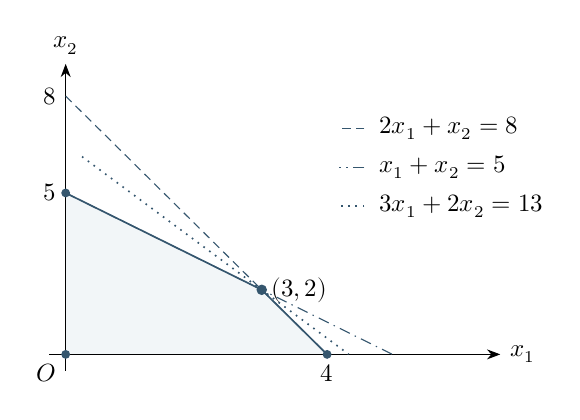
\begin{tikzpicture}[x=0.83cm,y=0.41cm]
\path[region] (0,0)--(4,0)--(3,2)--(0,5)--cycle;
\draw[axis] (-0.25,0)--(6.65,0) node[right] {$x_1$};
\draw[axis] (0,-0.5)--(0,9) node[above] {$x_2$};
\draw[helper] (0,8)--(4,0);
\draw[Theme,dash pattern=on 4pt off 2pt on 0.5pt off 2pt,thin] (0,5)--(5,0);
\draw[curve] (0,5)--(3,2)--(4,0);
\draw[Theme,dotted,semithick] (0.25,6.125)--(4.33,0.005);
\fill[Theme] (0,0) circle (1.6pt) (4,0) circle (1.6pt)
  (3,2) circle (1.9pt) (0,5) circle (1.6pt);
\node[below left] at (0,0) {$O$};
\node[below] at (4,0) {$4$};
\node[left] at (0,5) {$5$};
\node[left] at (0,8) {$8$};
\node[right] at (3,2) {$(3,2)$};
\node[anchor=west] at (4.65,7.0) {$2x_1+x_2=8$};
\node[anchor=west] at (4.65,5.8) {$x_1+x_2=5$};
\node[anchor=west] at (4.65,4.6) {$3x_1+2x_2=13$};
\draw[helper] (4.57,7)--(4.18,7);
\draw[Theme,dash pattern=on 4pt off 2pt on 0.5pt off 2pt,thin] (4.57,5.8)--(4.18,5.8);
\draw[Theme,dotted,semithick] (4.57,4.6)--(4.18,4.6);
\end{tikzpicture}
\diagramcaption{阴影为可行集，点线为通过最优点的目标等值线}
\end{center}

两条资源边界相减得到交点 $(3,2)$。最优性的代数验证是把资源限制直接相加
\[
  3x_1+2x_2=(2x_1+x_2)+(x_1+x_2)\le 8+5=13 .
\]
点 $(3,2)$ 使两条限制同时取等，因此最大利润为 $13$ 千元。若工时减为 $7$，上界降为 $12$ 千元，点 $(2,3)$ 使两条限制取等，恰好达到新上界。这一结论来自改变一个参数后的重新检验。

\subsection{0--1 背包与投资选址}
用 $x_j\in\{0,1\}$ 表示是否选择第 $j$ 件物品。设其质量为 $m_j$，价值为 $v_j$，允许总质量为 $W$，则
\[
  \max \sum_{j=1}^{n}v_jx_j,\qquad
  \sum_{j=1}^{n}m_jx_j\le W,\qquad x_j\in\{0,1\}.
\]
投资选址具有同一结构。将物品替换为候选站点，将质量替换为投资额，将价值替换为预期净收益，$W$ 即预算。若选址之间共享资源或相互依赖，还要按实际要求加入相应条件。

\begin{worked}{逐一检查背包的可行组合}
四件物品的质量依次为 $2,3,4,5$，价值依次为 $5,7,9,11$，容量为 $6$。求最优选择，并考察按单位质量价值顺序装入的结果。
\end{worked}
\sol
三件最轻物品的总质量为 $9$，因此可行方案最多选两件。所有单件方案均可行，价值最高为 $11$。可行的两件组合只有 $\{1,2\}$ 和 $\{1,3\}$，价值分别为 $12$ 和 $14$。最优选择为第 1、3 件，恰好用完容量。

按 $v_j/m_j$ 从高到低依次装入时，先选第 1、2 件，剩余容量为 $1$，得到价值 $12$。若将 $x_j\in\{0,1\}$ 放宽为 $0\le x_j\le 1$，则称为\term{连续松弛}。原可行方案都保留在松弛问题中，所以松弛的最大值是原最大值的上界。可行分装方案 $(1,1,\tfrac14,0)$ 的价值达到 $14.25$，其分数坐标在原模型中没有整件物品的解释。

\subsection{向量、子空间与投影}
本讲义使用列向量。$x\transpose y=\sum_i x_i y_i$ 是\term{内积}，$\norm{x}=\sqrt{x\transpose x}$ 是欧氏范数。$x\transpose y=0$ 表示正交。从 $x$ 沿非零向量 $d$ 移动写成 $x+td$，当 $t>0$ 时，移动距离为 $t\norm{d}$。若从距离出发指定步长，可先将方向除以 $\norm{d}$。

向量的比较按分量理解，例如 $x\le y$ 表示所有 $x_i\le y_i$，$x<y$ 表示所有 $x_i<y_i$。$\norm{x-y}$ 是两点距离，三角不等式 $\norm{x+y}\le\norm{x}+\norm{y}$ 保证经中间点的路程至少等于两点间直线距离。有限维中，$x^{(k)}\to x$ 等价于 $\norm{x^{(k)}-x}\to0$，也等价于各分量分别趋于 $x_i$。

$B_\varepsilon(x)=\{y:\norm{y-x}<\varepsilon\}$ 称为以 $x$ 为中心的开球。一个集合的内点能被完全包含在集内的小球包围。边界点的任意小球同时与该集合及其补集相交。开集中的点全是内点，闭集包含其收敛点列的极限。闭且有界的 $\R^n$ 中集合称为\term{紧集}，第二章将用到这个条件。

给定向量 $d_1,\ldots,d_k$，所有线性组合 $\sum_j\alpha_j d_j$（$\alpha_j\in\R$）组成\term{张成子空间} $L$。矩阵的秩等于其列空间的维数，抽取一组线性无关列可得到该列空间的一组基。子空间的\term{正交补}定义为
\[
  L^\perp=\{r\in\R^n:r\transpose u=0,\ \forall u\in L\}.
\]

\begin{infobox}{定理\quad 子空间投影}
任何 $z\in\R^n$ 可唯一分解为 $z=p+r$，其中 $p\in L$ 且 $r\in L^\perp$。$p$ 是 $L$ 上距离 $z$ 最近的点，最短距离为 $\norm{r}$。
\end{infobox}
取 $L$ 的标准正交基 $u_1,\ldots,u_k$，令 $p=\sum_j(u_j\transpose z)u_j$，则 $r=z-p$ 与每个 $u_j$ 正交，故 $r\in L^\perp$。对任意 $v\in L$，$p-v$ 与 $r$ 正交，因此
\[
  \norm{z-v}^2=\norm{r}^2+\norm{p-v}^2\ge \norm{r}^2 .
\]
仅当 $v=p$ 时等号成立。若 $L=\R^n$，则 $L^\perp=\{0\}$。若用非正交基的列组成满列秩矩阵 $U$，可写 $p=U\alpha$，用 $U\transpose(z-U\alpha)=0$ 求系数。

\begin{worked}{投影到过原点的一条直线}
将 $z=(3,1)\transpose$ 投影到 $L=\operatorname{span}\{d\}$，其中 $d=(1,1)\transpose$。求投影、残差和最短距离。
\end{worked}
\sol
设 $p=\alpha d$，由 $d\transpose(z-\alpha d)=0$ 得 $\alpha=d\transpose z/(d\transpose d)=2$。因此 $p=(2,2)\transpose$，$r=(1,-1)\transpose$，最短距离为 $\sqrt{2}$。

\Needspace{7.6\baselineskip}
\begin{center}
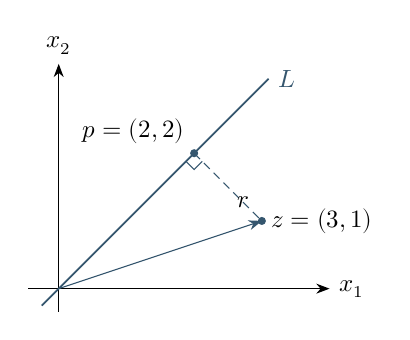
\begin{tikzpicture}[scale=0.86]
\draw[axis] (-0.45,0)--(4,0) node[right] {$x_1$};
\draw[axis] (0,-0.34)--(0,3.32) node[above] {$x_2$};
\draw[curve] (-0.25,-0.25)--(3.1,3.1) node[right] {$L$};
\draw[helper] (2,2)--(3,1);
\draw[Theme,thin] (1.88,1.88)--(2,1.76)--(2.12,1.88);
\draw[Theme,->] (0,0)--(3,1);
\fill[Theme] (2,2) circle (1.7pt) (3,1) circle (1.7pt);
\node[above left] at (2,2) {$p=(2,2)$};
\node[right] at (3,1) {$z=(3,1)$};
\node[below right] at (2.5,1.5) {$r$};
\end{tikzpicture}
\diagramcaption{投影点 $p$ 位于子空间上，残差 $r$ 垂直于子空间}
\end{center}

\subsection{对所有向量成立的内积不等式}
\begin{infobox}{定理\quad 从内积界推断分量和正交性}
设 $w\in\R^n$，$\alpha\in\R$。若 $w\transpose y\le\alpha$ 对所有 $y\ge0$ 成立，则 $w\le0$ 且 $\alpha\ge0$。若这一不等式对一个子空间 $L$ 的所有 $y$ 成立，则 $w\in L^\perp$ 且 $\alpha\ge0$。
\end{infobox}
两种情形都可代入 $y=0$ 得到 $\alpha\ge0$。在第一种情形代入 $y=t e_i$，其中 $e_i$ 为第 $i$ 个单位坐标向量，$t>0$。若 $w_i>0$，$t w_i$ 会超过任何固定上界。在第二种情形，若 $w\transpose u\ne0$，可在 $L$ 中取 $y=t u$，选择 $t$ 的正负并增大 $|t|$，使内积趋于 $+\infty$。当 $L=\R^n$ 时，结论为 $w=0$。

替换 $y$ 为 $-y$ 可以切换非正和非负向量的范围。将不等式两边乘以 $-1$ 可以转换上下界。例如 $w\transpose y\ge\alpha$ 对所有 $y\ge0$ 成立，等价于 $(-w)\transpose y\le-\alpha$，故 $w\ge0$ 且 $\alpha\le0$。

\subsection{多元函数、梯度和 Hesse 矩阵}
\begin{infobox}{定义\quad 一阶与二阶导数}
对标量函数 $f$，\term{梯度} $\nabla f(x)$ 是偏导数组成的列向量。若二阶偏导连续，\term{Hesse 矩阵} $\nabla^2 f(x)$ 是对称矩阵，其第 $i,j$ 项为 $\partial^2 f/\partial x_i\partial x_j$。梯度决定一阶变化，Hesse 矩阵给出各方向的二阶曲率。
\end{infobox}
仿射函数 $f(x)=c\transpose x+b$ 满足 $\nabla f=c$、$\nabla^2 f=0$。对向量值函数 $F(x)=Ax+b$，本讲义把每个输出分量的梯度转置排成一行，故 Jacobi 矩阵 $DF=A$。若按课件将这些梯度排成列，则所得矩阵为 $A\transpose$。

二次函数可取 $f(x)=\tfrac12 x\transpose Qx+c\transpose x+b$，其中 $Q=Q\transpose$。展开 $f(x+h)$ 后，一次项为 $(Qx+c)\transpose h$，二次项为 $\tfrac12 h\transpose Q h$，所以
\[
  \nabla f(x)=Qx+c,\qquad \nabla^2 f(x)=Q .
\]
若给定的 $Q$ 非对称，可先以 $\tfrac12(Q+Q\transpose)$ 替换。因为 $x\transpose Qx$ 是标量，转置后等于 $x\transpose Q\transpose x$，二次型保持原值。

\begin{worked}{由二次多项式读出梯度和 Hesse 矩阵}
设 $f(x)=x_1^2+2x_1x_2+3x_2^2-4x_1+2x_2$。求 $\nabla f(x)$、$\nabla^2 f(x)$，并算出在 $x=(1,0)\transpose$ 的梯度。
\end{worked}
\sol
分别对两个坐标求偏导，再对这两个结果求导，得到
\[
\nabla f(x)=
\begin{pmatrix}2x_1+2x_2-4\\2x_1+6x_2+2\end{pmatrix},
\qquad
\nabla^2 f(x)=\begin{pmatrix}2&2\\2&6\end{pmatrix},
\qquad
\nabla f(1,0)=(-2,4)\transpose .
\]
交叉项 $2x_1x_2$ 在 $\tfrac12 x\transpose Qx$ 中由 $Q_{12}$ 与 $Q_{21}$ 共同产生，所以这里 $Q_{12}=Q_{21}=2$。

\subsection{Taylor 展开与中值公式}
设 $x_0$ 位于 $f$ 的光滑区域内，$h=x-x_0$。$f$ 在 $x_0$ 可微时，一阶 Taylor 展开为
\[
  f(x_0+h)=f(x_0)+\nabla f(x_0)\transpose h+o(\norm{h}).
\]
若 $f$ 在 $x_0$ 附近二次连续可微，则有二阶展开
\begin{equation}\label{eq:taylor}
f(x_0+h)=f(x_0)+\nabla f(x_0)\transpose h
+\tfrac12 h\transpose\nabla^2 f(x_0)h+o(\norm{h}^2).
\end{equation}
两项导数都在展开点 $x_0$ 处计算。$o(\norm{h}^2)$ 表示余项除以 $\norm{h}^2$ 后，随 $h\to0$ 趋于零。

在连接 $x_0$ 和 $x_0+h$ 的线段上令 $\phi(t)=f(x_0+th)$。按链式法则，$\phi'(t)=\nabla f(x_0+th)\transpose h$，$\phi''(t)=h\transpose\nabla^2 f(x_0+th)h$。分别将一元中值定理和含 Lagrange 余项的 Taylor 公式用于 $\phi$，得到
\begin{align*}
f(x_0+h)&=f(x_0)+\nabla f(x_0+\theta h)\transpose h,\\
f(x_0+h)&=f(x_0)+\nabla f(x_0)\transpose h
+\tfrac12 h\transpose\nabla^2 f(x_0+\eta h)h .
\end{align*}
第一式在沿线段满足一元中值定理的条件时成立，第二式可在 $f$ 沿线段二次连续可微时使用。其中 $\theta,\eta\in(0,1)$ 各自存在，一般可以不同。式 \eqref{eq:taylor} 的二次项取在 $x_0$，中值形式的二阶导数取在线段内部。

\begin{worked}{辨认一阶和二阶近似的误差}
设 $f(x_1,x_2)=x_1+x_1x_2+2x_2^2+x_1^3$。求在原点的一阶和二阶近似，并与真实函数比较。
\end{worked}
\sol
在原点，$f=0$，$\nabla f=(1,0)\transpose$，$\nabla^2f=\begin{pmatrix}0&1\\1&4\end{pmatrix}$。令 $h=(h_1,h_2)\transpose$，一阶近似为 $h_1$，二阶近似为 $h_1+h_1h_2+2h_2^2$，后者的误差为 $h_1^3$。因 $|h_1^3|\le\norm{h}^3$，它是 $o(\norm{h}^2)$。沿 $h=(t,t)\transpose$，真实函数值为 $t+3t^2+t^3$，两种近似分别遗漏 $3t^2+t^3$ 和 $t^3$。

\clearpage
\subsection{本章练习}
本章练习的参考解答见第 \pageref{sec:answers} 页。
\begin{enumerate}[label=1.\arabic*.,ref=1.\arabic*,leftmargin=3em]
\item\label{ex:production} 两种产品产量 $x_1,x_2$ 可以取非负实数。第一、二种产品单位利润分别为 $4$、$3$，单位工时分别为 $2$、$1$，共有 $10$ 个工时。每件产品用一单位材料，材料上限为 $7$，第一种至少生产 $2$ 件。建立模型并求最优值。
\item\label{ex:yield} 两种产品的合格产出分别为 $6$ 吨和 $8$ 吨，产出投入比分别为 $0.6$ 和 $0.8$。计算总合格率。若题给的 $6$、$8$ 吨改指投入，两种产品合计的合格率是多少？分别判断是否达到 $71\%$。
\item\label{ex:choose} 三个项目的投资依次为 $2,3,4$，收益依次为 $4,7,9$，预算为 $6$。选项目 3 时必须选项目 1。写出 $0$--$1$ 模型，求最优组合。
\item\label{ex:proj} 将 $z=(2,1,1)\transpose$ 投影到由 $(1,1,0)\transpose$ 与 $(0,1,1)\transpose$ 张成的子空间。求投影与距离，并验证残差与两个基向量正交。
\item\label{ex:orth} 设 $w=(a,b,c)\transpose$，$L=\{y\in\R^3:y_1+y_2=0,\ y_3=0\}$。若 $w\transpose y\le2$ 对所有 $y\in L$ 成立，$a,b,c$ 有何限制？若再要求该式对所有 $y\ge0$ 成立，结论怎样变化？
\item\label{ex:quadratic} 设 $f(x)=\tfrac12x\transpose Qx$，其中 $Q=\begin{pmatrix}2&3\\1&4\end{pmatrix}$。写成坐标多项式，并求 $\nabla f(1,1)$ 与 $\nabla^2f$。
\item\label{ex:taylor} 设 $f(x_1,x_2)=x_1^2x_2+x_2^2$。在 $x_0=(1,1)\transpose$ 沿 $h=(s,t)\transpose$ 写出二阶 Taylor 展开，指出精确余项。
\end{enumerate}

\chapterpage{基本概念和理论基础}\label{sec:theory}
线性规划的可行集通常由若干半空间的交集给出。任取两个可行方案，它们的加权平均仍可行。这个性质称为凸性。它与目标函数的凸性结合时，能把局部的最优性结论推广到整个可行集。对于标准形线性规划，还可用极点和极方向描述全部可行方案。

\subsection{可行解、全局最优解与局部最优解}
以下以最小化为例。课件用 $(f,S)$ 指以 $f$ 为目标、以 $S$ 为可行集的问题。本讲义常将约束展开为
\[
\begin{aligned}
\min_{x\in\R^n}\quad & f(x)\\
\text{s.t.}\quad & g_i(x)\le0,\quad i=1,\ldots,m,\\
& h_j(x)=0,\quad j=1,\ldots,\ell .
\end{aligned}
\]
把各 $g_i$ 排成向量 $g(x)$、各 $h_j$ 排成向量 $h(x)$，可缩写为 $S=\{x:g(x)\le0,\ h(x)=0\}$。所有不等式逐分量成立。

\begin{infobox}{定义\quad 全局最优、局部最优与最优值}
若 $x^\star\in S$，且 $f(x^\star)\le f(x)$ 对所有 $x\in S$ 成立，则 $x^\star$ 是\term{全局最优解}。若存在 $\varepsilon>0$，使此式对所有 $x\in S\cap B_\varepsilon(x^\star)$ 成立，则 $x^\star$ 是\term{局部最优解}。

对于相应比较范围内每个 $x\ne x^\star$，若都有 $f(x^\star)<f(x)$，则称为\term{严格}全局或局部最优解。全局最优解对应的数 $f^\star=f(x^\star)$ 称为\term{最优值}。
\end{infobox}
全局最优解必为局部最优解。遇到边界点时，局部比较只在球内的可行点之间进行。最优解可以有多个，例如 $f(x)=0$ 在 $S=[0,1]$ 上的每个点都全局最优，此时最优值只有一个。

\begin{worked}{同一目标中出现两个局部最低点}
设 $S=\R$，$f(x)=x^4/4-x^3/3-x^2$。判断其严格局部最优解与全局最优解。
\end{worked}
\sol
$f'(x)=x(x-2)(x+1)$ 在区间 $(-\infty,-1)$、$(-1,0)$、$(0,2)$ 和 $(2,\infty)$ 上的符号依次为 $-,+,-,+$。因此 $-1$ 和 $2$ 都是严格局部最小点，$0$ 是局部极大点。又因为 $f(x)\to+\infty$（$|x|\to\infty$），只需比较两个局部最小值。$f(-1)=-5/12$，$f(2)=-8/3$，所以 $2$ 是严格全局最优解。

\Needspace{9\baselineskip}
\begin{center}
\begin{tikzpicture}[x=1.55cm,y=0.68cm]
\draw[axis] (-1.95,0)--(3.10,0) node[right] {$x$};
\draw[axis] (0,-3.18)--(0,1.76) node[above] {$f(x)$};
\draw[curve,domain=-1.75:2.91,samples=100,smooth]
  plot (\x,{(\x*\x*\x*\x)/4-(\x*\x*\x)/3-\x*\x});
\fill[Theme] (-1,-5/12) circle (1.8pt) (2,-8/3) circle (1.8pt);
\node[below left] at (-1,-5/12) {$(-1,-5/12)$};
\node[below right] at (2,-8/3) {$(2,-8/3)$};
\end{tikzpicture}
\diagramcaption{两个局部最小值中，右侧的值更低}
\end{center}

\begin{infobox}{定理\quad 连续函数何时一定能取到最值}
若 $S\subseteq\R^n$ 非空且紧，$f$ 在 $S$ 上连续，则 $f$ 在 $S$ 上都能取到最大值和最小值。
\end{infobox}
例如 $\min\{x:0<x\le1\}$ 的下确界是 $0$，但 $0$ 被可行集排除，因而没有最优解。$\min\{x:x\in\R\}$ 的目标值向下无界。非紧集上也可能有最优解，例如 $x^2$ 在 $\R$ 上于 $0$ 处取到最小值。判断最优解的存在性和判断某个候选点的最优性是两个步骤。

\subsection{凸集、凸组合与单纯形}
\begin{infobox}{定义\quad 凸集}
若对任意 $x,y\in S$ 和 $\theta\in[0,1]$，都有 $\theta x+(1-\theta)y\in S$，则 $S$ 为\term{凸集}。系数 $\theta$ 从 $0$ 变到 $1$ 时，新点沿着从 $y$ 到 $x$ 的线段移动。空集与单点集均满足定义。
\end{infobox}

\Needspace{11\baselineskip}
\begin{center}
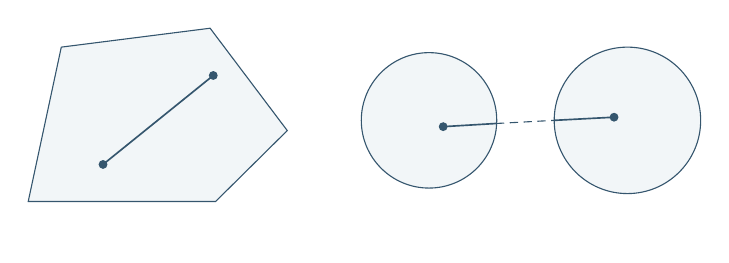
\begin{tikzpicture}
\path[draw=Theme,region] (-4,0.18)--(-3.58,2.14)--(-1.69,2.38)
  --(-0.71,1.08)--(-1.62,0.18)--cycle;
\draw[curve] (-3.05,0.65)--(-1.65,1.78);
\fill[Theme] (-3.05,0.65) circle (1.6pt) (-1.65,1.78) circle (1.6pt);
\node[below] at (-2.35,0) {凸集};
\path[draw=Theme,region] (1.09,1.21) circle (0.86);
\path[draw=Theme,region] (3.61,1.21) circle (0.93);
\draw[curve] (1.27,1.13)--(1.94,1.17) (2.68,1.21)--(3.44,1.25);
\draw[helper] (1.94,1.17)--(2.68,1.21);
\fill[Theme] (1.27,1.13) circle (1.6pt) (3.44,1.25) circle (1.6pt);
\node[below] at (2.35,0) {非凸集};
\end{tikzpicture}
\diagramcaption{右图中的两点分处不同圆盘，线段的虚线部分落在集合外}
\end{center}

\begin{worked}{用定义判断线性等式的解集}
证明 $S=\{x\in\R^n:Ax=b\}$ 为凸集。
\end{worked}
\sol
取 $x,y\in S$，则 $Ax=Ay=b$。由矩阵乘法的线性性，
\[
 A\bigl(\theta x+(1-\theta)y\bigr)=\theta b+(1-\theta)b=b .
\]
因此整个线段都在 $S$ 内。对 $a\transpose x\le b$，同样计算可得到
$a\transpose\bigl(\theta x+(1-\theta)y\bigr)\le b$，故闭半空间也是凸集。

对点 $x^{(1)},\ldots,x^{(k)}$，若 $\lambda_i\ge0$ 且 $\sum_{i=1}^k\lambda_i=1$，则 $\sum_{i=1}^k\lambda_i x^{(i)}$ 称为一个\term{凸组合}。线段定义等价于任意有限多个点的凸组合仍在集合中。证明可按点数归纳。若最后一项系数 $\lambda_k<1$，先用权重 $\lambda_i/(1-\lambda_k)$ 合并前 $k-1$ 点，再把所得点与 $x^{(k)}$ 用两点定义合并。若 $\lambda_k=1$，组合就是 $x^{(k)}$。

给定有限点集，所有凸组合构成它的\term{凸包}，记作 $\conv\{x^{(1)},\ldots,x^{(k)}\}$。凸包是包含给定点的最小凸集。课件把有限点的凸包称为\term{多胞形}。若 $x^{(i)}-x^{(1)}$（$i=2,\ldots,k$）线性无关，则这些点仿射无关，凸包称为 $(k-1)$ 维\term{单纯形}。例如非共线三点的凸包是三角形，四个仿射无关点在 $\R^3$ 中给出四面体。在 $\R^n$ 中，单纯形至多由 $n+1$ 个仿射无关点生成。

\begin{worked}{用凸组合坐标描述一个三角形}
给定 $v_1=(0,0)\transpose$、$v_2=(2,0)\transpose$、$v_3=(0,3)\transpose$。写出凸包的不等式描述，并找出点 $(1,1)\transpose$ 的凸组合系数。
\end{worked}
\sol
对 $x=\sum_i\lambda_i v_i$，有 $x_1=2\lambda_2$、$x_2=3\lambda_3$，因此
\[
x_1\ge0,\quad x_2\ge0,\quad x_1/2+x_2/3\le1 .
\]
反过来，满足这些式子的 $x$ 对应 $\lambda_2=x_1/2$、$\lambda_3=x_2/3$、$\lambda_1=1-\lambda_2-\lambda_3$，三者都非负且和为 $1$。点 $(1,1)\transpose$ 的系数为 $(1/6,1/2,1/3)$，全为正，说明它位于三角形内部。

\subsection{凸集的交、内点、闭包与分离}
任意多个凸集的交仍是凸集，因为交集中的两点在每个集合内都能连成线段。并集则要单独检验，例如 $[-2,-1]\cup[1,2]$ 缺少连接 $-1$ 与 $1$ 的中点 $0$。

设 $S$ 凸。若 $x,y$ 都是内点，取公共半径 $r>0$，使它们周围两个半径 $r$ 的开球都在 $S$ 内。对任意 $\norm{u}<r$，点 $\theta(x+u)+(1-\theta)(y+u)$ 在 $S$ 内，因此组合点周围也有一个半径 $r$ 的开球。于是内点集为凸集。对闭包中的 $x,y$ 分别取来自 $S$ 的收敛点列，其对应凸组合在 $S$ 中，极限是 $\theta x+(1-\theta)y$，所以闭包也为凸集。

这两个性质的逆命题都可由反例检验。$[-2,-1]\cup\{1\}$ 的内点集为 $(-2,-1)$，但从 $-1$ 到 $1$ 的线段有缺口。$[0,1]\setminus\{1/2\}$ 的闭包为 $[0,1]$，但删除的 $1/2$ 恰是两个端点的中点。

对 $a\ne0$，集合 $\{x:a\transpose x=b\}$ 是\term{超平面}，$a$ 给出法向量。它将空间划分为 $a\transpose x\le b$ 与 $a\transpose x\ge b$ 两个闭半空间。在二维中，超平面就是直线。

\begin{infobox}{定理\quad 支撑与分离}
对非空凸集 $C$ 的边界点 $p$，存在超平面经过 $p$，使 $C$ 限于它的一侧。例如选取适当 $a\ne0$，使 $a\transpose x\le a\transpose p$ 对所有 $x\in C$ 成立。这称为\term{支撑超平面}。

若两个非空凸集 $C,D$ 不相交，则存在 $a\ne0$ 和 $b$，使 $a\transpose x\le b\le a\transpose y$ 对所有 $x\in C,y\in D$ 成立。这称为\term{分离超平面}，等号可以出现。
\end{infobox}

\Needspace{11\baselineskip}
\begin{center}
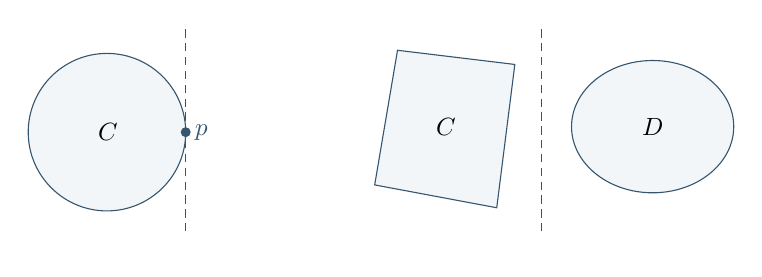
\begin{tikzpicture}
\path[draw=Theme,region] (-3.16,1.20) circle (1);
\draw[helper] (-2.16,-0.06)--(-2.16,2.52);
\fill[Theme] (-2.16,1.20) circle (1.8pt) node[right] {$p$};
\node at (-3.16,1.2) {$C$};
\node[below] at (-2.95,-0.04) {支撑};
\path[draw=Theme,region] (0.24,0.53)--(1.79,0.24)--(2.02,2.06)--(0.53,2.24)--cycle;
\path[draw=Theme,region] (3.77,1.27) ellipse (1.03 and 0.84);
\draw[helper] (2.36,-0.06)--(2.36,2.52);
\node at (1.14,1.26) {$C$};
\node at (3.77,1.27) {$D$};
\node[below] at (2.36,-0.04) {分离};
\end{tikzpicture}
\diagramcaption{左图的直线经过边界点，右图的直线将两集合放在两侧}
\end{center}

例如单位闭圆盘在 $p=(1,0)\transpose$ 的右支撑直线为 $x_1=1$。区间 $C=[-1,0]$ 与 $D=(0,1]$ 可由 $x=0$ 分离，$C$ 的端点恰好落在分离面上。若进一步要求两侧各留出正的间隔，就需要额外条件，此例的两个集合相距为零。若两集合都在同一超平面上，例如平面内同一直线上的两条不交线段，这条直线也满足弱分离的不等式。

\subsection{锥、凸锥与三种组合}
若 $x\in K$ 且 $t>0$ 时总有 $tx\in K$，课件称 $K$ 为以原点为顶点的\term{锥}。若 $K$ 同时为凸集，便是\term{凸锥}。例如 $\{0\}$、$\R^n$、$\R^n_+=\{x:x\ge0\}$ 都是凸锥。按课件对 $t>0$ 的约定，锥可不含原点，例如 $\{t v:t>0\}$，其中 $v\ne0$。

凸锥对\term{半正组合}封闭，即允许 $\lambda_i\ge0$ 且 $\sum_i\lambda_i>0$。因为可以先除以总权重做凸组合，再乘回总权重。反向取一个点即可得到正倍数封闭，取两个点且权重和等于 $1$ 即得凸性。本讲义用 $\cone\{v_i\}$ 表示允许全零权重的非负组合，因此生成的锥包含原点。后文的衰退锥也包含原点。

\begin{center}
\begin{tabularx}{\linewidth}{l l Y}
\toprule
组合形式 $\sum_i\lambda_i v_i$ & 系数条件 & 取尽所有系数得到\\
\midrule
线性组合 & $\lambda_i\in\R$ & 张成子空间\\
凸组合 & $\lambda_i\ge0,\ \sum_i\lambda_i=1$ & 凸包\\
非负组合 & $\lambda_i\ge0$ & 包含原点的生成锥\\
\bottomrule
\end{tabularx}
\end{center}
对 $v_1=(1,0)\transpose,v_2=(0,1)\transpose$，三个结果依次为全平面、连接二者的线段和第一象限（含坐标轴）。从固定两点换成任意多点时，系数条件保持相同含义。

\subsection{凸函数、严格凸函数与下水平集}
\begin{infobox}{定义\quad 凸函数与严格凸函数}
设 $S$ 为凸集，$f:S\to\R$。若对任意 $x,y\in S$ 和 $\theta\in[0,1]$，都有
\[
 f\bigl(\theta x+(1-\theta)y\bigr)\le\theta f(x)+(1-\theta)f(y),
\]
则 $f$ 为\term{凸函数}。若 $x\ne y$ 且 $0<\theta<1$ 时不等式恒严格，则 $f$ 为\term{严格凸函数}。$-f$ 为凸函数时，称 $f$ 为\term{凹函数}。
\end{infobox}
左边是中间点的真实函数值，右边是两端函数值沿弦线插值得到的高度。仿射函数处处取等，因而既凸又凹。严格凸要求每条非平凡弦线上的内部点高于相应的函数图像。

\Needspace{11\baselineskip}
\begin{center}
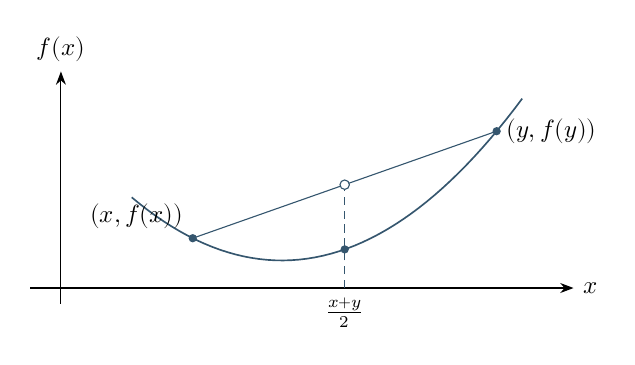
\begin{tikzpicture}[x=1.55cm,y=1.0cm]
\draw[axis] (-0.78,0)--(3.67,0) node[right] {$x$};
\draw[axis] (-0.53,-0.2)--(-0.53,2.75) node[above] {$f(x)$};
\draw[curve,domain=0.05:3.25,samples=50] plot (\x,{0.53*(\x-1.28)*(\x-1.28)+0.35});
\coordinate (U) at (0.55,0.632437);
\coordinate (V) at (3.04,1.991728);
\coordinate (A) at (1.795,1.3120825);
\coordinate (M) at (1.795,0.49056925);
\draw[Theme] (U)--(V);
\draw[helper] (1.795,0)--(A);
\fill[Theme] (U) circle (1.5pt) (V) circle (1.5pt) (M) circle (1.5pt);
\filldraw[draw=Theme,fill=white] (A) circle (1.7pt);
\node[above left] at (U) {$(x,f(x))$};
\node[right] at (V) {$(y,f(y))$};
\node[above left] at (A) {弦线上高度};
\node[right] at (1.89,0.32) {中点的函数值};
\node[below] at (1.795,0) {$\frac{x+y}{2}$};
\end{tikzpicture}
\diagramcaption{严格凸函数在两点之间的图像低于连接它们的弦线}
\end{center}

两点不等式可推广到有限凸组合，得到 Jensen 不等式
\[
 f\left(\sum_{i=1}^k\lambda_i x^{(i)}\right)
 \le \sum_{i=1}^k\lambda_i f(x^{(i)}),
 \qquad \lambda_i\ge0,\quad \sum_{i=1}^k\lambda_i=1.
\]
证明沿用有限凸组合的归纳法，在每次合并时应用两点不等式。取 $k=2$ 又回到凸函数的定义。

在共同凸定义域上，凸函数的非负线性组合仍凸，因为可以给每条凸性不等式乘非负系数后相加。点对点的最大值 $F(x)=\max_i f_i(x)$ 也凸，每个 $f_i$ 在组合点的值都不超过 $\theta F(x)+(1-\theta)F(y)$，故取最大值后仍满足此上界。

\begin{worked}{检验相减和取最小值}
给出反例，检验两个凸函数的差和逐点最小值能否保证凸。
\end{worked}
\sol
$x^2$ 与 $2x^2$ 都凸，取差得到 $-x^2$，在 $-1,1$ 的中点 $0$ 处取值 $0$，高于端点平均值 $-1$。取 $f_1(x)=(x-1)^2$ 和 $f_2(x)=(x+1)^2$，则 $\min\{f_1,f_2\}$ 在 $-1,1$ 均为 $0$，在中点为 $1$，也违反凸性不等式。

\term{下水平集}（课件简称水平集）为 $S_\alpha=\{x\in S:f(x)\le\alpha\}$。若 $f$ 凸，两个函数值均不超过 $\alpha$ 的点，它们的凸组合也满足相同上界，因此每个 $S_\alpha$ 都凸。反向检验可用阶跃函数 $f(x)=0$（$x<0$）和 $f(x)=1$（$x\ge0$）。它的下水平集依次可能为空集、$(-\infty,0)$ 或 $\R$，全部凸。取 $-1,1$ 比较中点时，$f(0)=1>1/2$，函数不凸。

有限值凸函数在定义域的内点连续，边界可能出现跳跃。例如在 $[-1,1]$ 上，令 $f(x)=x^2$（$|x|<1$）而 $f(-1)=f(1)=2$。两点真凸组合落在区间内部时，$x^2$ 的凸性已给出所需上界，而提高端点值只会抬高右端。当凸组合落在端点时，参与组合的点都等于该端点。故函数仍凸，且 $\lim_{x\uparrow1}f(x)=1$ 与 $f(1)=2$ 不等。

\subsection{方向导数、梯度和可行方向}
在点 $x$ 处，若 $d\ne0$ 且 $x+td\in S$ 对充分小的 $t>0$ 成立，称 $d$ 为该点的\term{可行方向}。沿方向的局部变化率采用右极限
\begin{equation}\label{eq:directional}
 f'(x;d)=\lim_{t\downarrow0}\frac{f(x+td)-f(x)}{t}.
\end{equation}
若 $f$ 在 $x$ 的邻域可微，则一阶展开给出 $f'(x;d)=\nabla f(x)\transpose d$。这个值按参数 $t$ 计量。若按走过的单位距离计量，应取 $u=d/\norm{d}$，此时导数为 $\nabla f(x)\transpose u$。

当梯度非零时，$\nabla f(x)\transpose u=\norm{\nabla f(x)}\cos\vartheta$，其中 $\vartheta$ 是梯度与单位向量 $u$ 的夹角。在所有单位方向中，梯度方向取得最大值 $\norm{\nabla f(x)}$，反向取得最小值 $-\norm{\nabla f(x)}$。若一条可微曲线始终保持相同函数值，在曲线上求导可知它在 $x$ 处的切向量与梯度正交。

\begin{worked}{同一点的上升、下降与等值线切向}
设 $f(x)=x_1^2+2x_2^2$，在 $p=(1,1)\transpose$ 处求沿 $d=(1,-1)\transpose$ 的方向导数，并找一个与等值线相切的方向。
\end{worked}
\sol
$\nabla f(p)=(2,4)\transpose$，所以 $f'(p;d)=-2$。沿该方向每单位距离的变化率为 $-\sqrt{2}$。向量 $(2,-1)\transpose$ 与梯度的内积为 $0$，因此沿椭圆 $x_1^2+2x_2^2=3$ 的切线方向。加入 $x_1\ge1$ 时，点 $p$ 处的负梯度会立即进入 $x_1<1$ 的区域。可行方向 $(0,-1)\transpose$ 仍使目标值一阶下降，变化率为 $-4$。

\Needspace{12\baselineskip}
\begin{center}
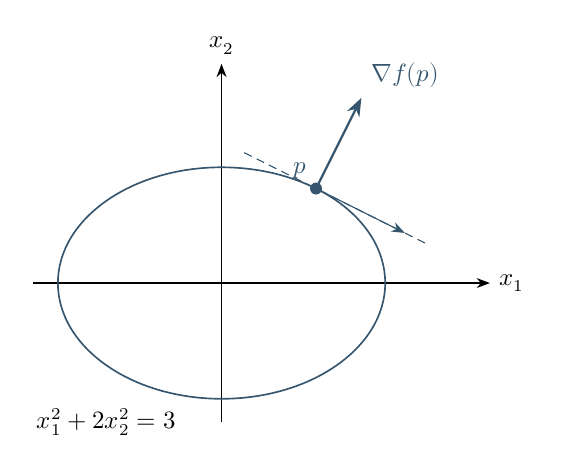
\begin{tikzpicture}[scale=1.2]
\draw[axis] (-2.0,0)--(2.84,0) node[right] {$x_1$};
\draw[axis] (0,-1.47)--(0,2.32) node[above] {$x_2$};
\draw[curve] (0,0) ellipse (1.732 and 1.225);
\draw[helper] (0.24,1.38)--(2.18,0.41);
\draw[Theme,->,thick] (1,1)--(1.48,1.96) node[above right] {$\nabla f(p)$};
\draw[Theme,->] (1,1)--(1.94,0.53) node[right] {切向};
\fill[Theme] (1,1) circle (1.8pt) node[above left] {$p$};
\node at (-1.22,-1.47) {$x_1^2+2x_2^2=3$};
\end{tikzpicture}
\diagramcaption{在 $p$ 点，梯度垂直于等值线的切线}
\end{center}

凸性还保证可行方向上的右导数在扩展实数意义下存在。令 $\phi(t)=f(x+td)$，直线上的限制仍凸。若 $0<s<t$ 且两点可行，将 $s$ 写成 $0$ 与 $t$ 的凸组合，得到
\[
  \frac{\phi(s)-\phi(0)}{s}\le
  \frac{\phi(t)-\phi(0)}{t}.
\]
所以从右侧趋近零时，差商单调向其下确界靠近。边界处可能得到 $-\infty$，例如 $f(x)=-\sqrt{x}$ 在 $[0,\infty)$ 上凸，$f'(0;1)=\lim_{t\downarrow0}(-1/\sqrt{t})=-\infty$。

\subsection{一阶与二阶凸性判别}
\begin{infobox}{定理\quad 梯度判别与 Hesse 矩阵判别}
设 $S$ 为非空开凸集，$f$ 在 $S$ 上可微。$f$ 凸当且仅当对任意 $x,y\in S$，
\begin{equation}\label{eq:gradient-bound}
 f(y)\ge f(x)+\nabla f(x)\transpose(y-x).
\end{equation}
若 $f$ 在 $S$ 上二次连续可微，$f$ 凸当且仅当对所有 $x\in S$ 有 $\nabla^2 f(x)\succeq0$。若对所有 $x\in S$ 有 $\nabla^2 f(x)\succ0$，则 $f$ 严格凸。
\end{infobox}

若 $f$ 凸，以 $d=y-x$ 代入方向差商的单调关系，取 $t=1$ 并令 $s\downarrow0$，即得式 \eqref{eq:gradient-bound}。反向设 $z=\theta x+(1-\theta)y$，分别在 $z$ 处对 $x,y$ 应用式 \eqref{eq:gradient-bound}，再分别乘 $\theta,1-\theta$ 后相加。两项一阶变化抵消，因为 $\theta(x-z)+(1-\theta)(y-z)=0$，余下的正是凸性不等式。

对二阶判别，沿任意线段令 $\phi(t)=f(x+td)$，有 $\phi''(t)=d\transpose\nabla^2 f(x+td)d$。Hesse 矩阵半正定时，每条线段上的 $\phi''$ 非负，由一元判别知 $\phi$ 凸，因而 $f$ 凸。反向沿任意方向检查凸函数的二阶导数，均得 $d\transpose\nabla^2 f(x)d\ge0$。Hesse 矩阵处处正定时，任意非平凡线段上的二阶导数为正，给出严格凸性。严格凸函数也允许某点二阶导数为零，例如 $f(x)=x^4$ 的一阶导数严格递增，而 $f''(0)=0$。

对称矩阵 $H$ 的符号由二次型 $d\transpose Hd$ 决定。若对所有 $d\ne0$ 均大于零，记作 $H\succ0$。若均大于等于零，记作 $H\succeq0$。负定、半负定可对 $-H$ 作相应判断。正定可用特征值全正或顺序主子式全正判定，半正定可用特征值全非负或\term{全部}主子式非负判定。对称 $2\times2$ 矩阵 $\begin{pmatrix}a&b\\b&c\end{pmatrix}$ 半正定的条件是 $a\ge0,\ c\ge0,\ ac-b^2\ge0$。

\begin{worked}{判定三类二次函数的凸凹性}
依次判断下列函数。第三个函数分别取 $a=5$ 与 $a=4.5$。
\begin{align*}
f_1(x)&=x_1^2+2x_1x_2+2x_2^2+10x_1-4,\\
f_2(x)&=-3x_1^2+x_1x_2-x_2^2-2x_3^2-2x_2x_3+26,\\
f_3(x)&=3x_1^2+a x_1x_2+2x_2^2-4x_1+6 .
\end{align*}
\end{worked}
\sol
三个函数的 Hesse 矩阵分别为
\[
H_1=\begin{pmatrix}2&2\\2&4\end{pmatrix},\qquad
H_2=\begin{pmatrix}-6&1&0\\1&-2&-2\\0&-2&-4\end{pmatrix},\qquad
H_3=\begin{pmatrix}6&a\\a&4\end{pmatrix}.
\]
$H_1$ 的顺序主子式为 $2,4$，故正定，$f_1$ 严格凸。$H_2$ 的顺序主子式为 $-6,11,-20$，故 $-H_2$ 的顺序主子式全正，$f_2$ 严格凹。$H_3$ 的行列式为 $24-a^2$。当 $a=5$ 时行列式为 $-1$，两个特征值异号，$f_3$ 既非凸也非凹。当 $a=4.5$ 时行列式为 $15/4$ 且首个顺序主子式为 $6$，故 $f_3$ 严格凸。

\subsection{凸规划与全局最优性}
在\term{凸规划}中，最小化的目标函数在可行集上凸，且可行集本身凸。常见的充分条件是目标 $f$ 和每个 $g_i$ 都凸，等式 $h_j$ 为仿射函数。理由是各下水平集 $\{x:g_i(x)\le0\}$ 和各仿射等式的解集都凸，它们的交集仍凸。对于最大化，可先把目标取负再检查凸性。给约束改写方向后，须检验最终位于 $\le0$ 左边的函数。

\begin{infobox}{定理\quad 凸规划的局部最优解也是全局最优解}
设 $S$ 为凸集，$f$ 在 $S$ 上凸。若 $x^\star$ 是最小化问题的局部最优解，则它也是全局最优解。若 $f$ 严格凸且最优解存在，则最优解唯一。
\end{infobox}
若有可行点 $y$ 满足 $f(y)<f(x^\star)$，对任意 $0<t<1$，$z_t=(1-t)x^\star+ty$ 可行，且
\[
f(z_t)\le(1-t)f(x^\star)+tf(y)<f(x^\star).
\]
取充分小的 $t$，$z_t$ 就在 $x^\star$ 的任意给定邻域内，与局部最优矛盾。若有两个不同的全局最优点，严格凸性会使它们的中点取得更小值，也产生矛盾。严格凸性负责唯一性，存在性仍须另验，例如 $e^x$ 在 $\R$ 上严格凸，下确界为 $0$，没有点取到它。

若 $f$ 在包含 $S$ 的开凸邻域上凸且可微，则对 $x^\star\in S$ 有如下判据
\begin{equation}\label{eq:optcond}
 x^\star\text{ 全局最优}\quad\Longleftrightarrow\quad
 \nabla f(x^\star)\transpose(y-x^\star)\ge0\quad\text{对所有 }y\in S.
\end{equation}
必要性来自沿 $x^\star$ 到 $y$ 的可行线段取右导数，局部最优时该导数非负。充分性来自式 \eqref{eq:gradient-bound}，一阶下界已经至少等于 $f(x^\star)$。若 $x^\star$ 是内点，可取每个坐标轴的正反方向，因此 $\nabla f(x^\star)=0$。边界上使用式 \eqref{eq:optcond} 即可。例如 $f(x_1,x_2)=x_1^2+2x_2^2$ 在 $S=\{x:x_1\ge1\}$ 上，$x^\star=(1,0)\transpose$ 的梯度为 $(2,0)\transpose$，对各可行 $y$ 都有 $2(y_1-1)\ge0$，故 $x^\star$ 全局最优。

\begin{worked}{在一条线段上最小化严格凸函数}
最小化 $x_1^2+2x_2^2$，约束为 $x_1+x_2=1$、$x_1,x_2\ge0$。证明这是凸规划并求解。
\end{worked}
\sol
Hesse 矩阵为 $\operatorname{diag}(2,4)\succ0$，约束给出凸线段。消去 $x_2$ 得到 $u(t)=t^2+2(1-t)^2$，$0\le t\le1$。由 $u'(t)=6t-4=0$ 得 $t=2/3$，且 $u''(t)=6>0$。故唯一最优解为 $(2/3,1/3)\transpose$，最优值为 $2/3$。在原坐标中，该点梯度为 $(4/3,4/3)\transpose$，与线段方向 $(1,-1)\transpose$ 正交，也符合式 \eqref{eq:optcond}。

\subsection{多面体、极点与衰退方向}
\term{多面体}是有限个闭半空间的交集。等式 $a\transpose x=b$ 可用 $a\transpose x\le b$ 与 $-a\transpose x\le-b$ 两个不等式表达。因此
\begin{equation}\label{eq:standard}
  P=\{x\in\R^n:Ax=b,\ x\ge0\}
\end{equation}
是多面体，称为\term{标准形}。线性规划中可对约束 $Gx\le b$ 加入非负的\term{松弛变量} $s=b-Gx$，得到等式 $Gx+s=b$。二维非空多面体可以是有界多边形，也可以是无界区域、直线、线段或单点。

\begin{infobox}{定义\quad 极点与极方向}
若 $x\in P$ 无法写成 $P$ 中两个不同点的严格凸组合 $x=\theta u+(1-\theta)v$（$0<\theta<1$），则 $x$ 为 $P$ 的\term{极点}，对多面体也称顶点。

若 $d\ne0$，且对所有 $x\in P,t\ge0$ 都有 $x+td\in P$，则称 $d$ 为 $P$ 的\term{衰退方向}，课件简称方向。把零向量也纳入，得到衰退锥 $\operatorname{rec}P$。若 $d=d_1+d_2$ 且 $d_1,d_2\in\operatorname{rec}P$ 时，两项都只能为 $d$ 的非负倍数，则 $d$ 为\term{极方向}。同一极方向的正倍数组成一条\term{极射线}。
\end{infobox}
极点的判断要看能否在集合内选出一条线段，使候选点落在线段内部。正方形的顶角是极点，边的中点可写成两个顶角的平均值。可行方向只要求从当前点走一小段仍可行。衰退方向要求沿同一方向一直走，例如从区间 $[0,1]$ 的中点向右可走小步，区间的衰退锥却只有零向量。

若 $P=\{x:Gx\le q\}$ 非空，代入 $x+td$ 可知 $\operatorname{rec}P=\{d:Gd\le0\}$。充分性由 $G(x+td)=Gx+tGd\le q$ 直接得到。必要性只需从一个可行点出发，若 $Gd$ 某分量为正，增大 $t$ 就会越过该行上界。这也解释了课件从一个点出发检查所有步长的写法。对标准形 \eqref{eq:standard}，
\begin{equation}\label{eq:recession}
\operatorname{rec}P=\{d:Ad=0,\ d\ge0\}.
\end{equation}
其中 $Ad=0$ 使等式右端保持 $b$。若 $d_i<0$，只要步长足够大，$x_i+td_i$ 就会违反非负性。

\subsection{从基矩阵找极点}
设 \eqref{eq:standard} 中 $A$ 有 $m$ 行、$n$ 列且 $\rank A=m$。选 $m$ 根线性无关列组成可逆方阵 $B$，称为一个\term{基}，其余列组成 $N$。分别用 $x_B,x_N$ 记与这两个列块相对应的坐标。置 $x_N=0$，解 $Bx_B=b$，得到\term{基本解}。若基本解所有分量均非负，称为\term{基本可行解}。

\begin{infobox}{定理\quad 极点的两种判定}
设 $x\in P$，$I=\{i:x_i>0\}$，$A_I$ 由 $A$ 中第 $i\in I$ 列组成。以下条件等价。
\begin{enumerate}[label=\arabic*.,leftmargin=2em]
\item $x$ 是 $P$ 的极点。
\item $A_I$ 的列线性无关。
\item 存在一个基 $B$，使 $x_N=0$ 且 $x_B=B^{-1}b\ge0$。
\end{enumerate}
\end{infobox}
若 $A_I$ 的列线性相关，可找到非零向量 $u$，在 $I$ 外分量为零且 $Au=0$。取充分小的 $\varepsilon>0$，$x+\varepsilon u$ 与 $x-\varepsilon u$ 都保持非负，也满足等式。$x$ 是这两点的中点，因此不能是极点。

若 $A_I$ 列线性无关，假设 $x=\theta v+(1-\theta)w$ 且 $v,w\in P$、$0<\theta<1$。在 $I$ 外有 $x_i=0$，非负性迫使 $v_i=w_i=0$。由 $A_I(v_I-w_I)=0$ 得 $v_I=w_I$，所以两点重合。将 $A_I$ 的列补成基即可得到第 3 项。反过来，第 3 项的正分量对应列都是某个基的子集，因而线性无关。

最多有 $\binom{n}{m}$ 种基列候选。奇异候选、出现负分量的基本解应剔除。若基本可行解的某个基变量为零，称为\term{退化}。不同的基在退化时可能给出同一个极点，因此列出候选点后还要去重。

\begin{worked}{求含三个松弛变量的多面体的全部极点}
沿用第 2 章课件的数据。设 $x\in\R^5$ 且 $x\ge0$，满足
\[
A x=b,\qquad
A=\begin{pmatrix}3&2&1&0&0\\2&1&0&1&0\\0&3&0&0&1\end{pmatrix},
\qquad b=\begin{pmatrix}65\\40\\75\end{pmatrix}.
\]
求所有极点，并用 $x_1,x_2$ 平面验证。
\end{worked}
\sol
记 $A$ 的列为 $a_1,\ldots,a_5$。第 $3,4,5$ 列为单位矩阵的三列，因此 $\rank A=3$。每次选三列为候选，使其余变量为零。例如对候选 $(1,2,5)$，令 $x_3=x_4=0$。先用前两行 $3x_1+2x_2=65$ 和 $2x_1+x_2=40$ 求得 $x_1=15,x_2=10$，再由第三行得 $x_5=45$。

\Needspace{14\baselineskip}
\begin{center}
\small
\begin{tabularx}{\linewidth}{c l Y}
\toprule
候选列号 & 按 $(x_1,x_2,x_3,x_4,x_5)$ 写出的基本解 & 检验结果\\
\midrule
$(1,2,3)$ & $(15/2,25,-15/2,0,0)$ & $x_3<0$\\
$(1,2,4)$ & $(5,25,0,5,0)$ & 极点\\
$(1,2,5)$ & $(15,10,0,0,45)$ & 极点\\
$(1,3,4)$ & 无 & 候选列相关\\
$(1,3,5)$ & $(20,0,5,0,75)$ & 极点\\
$(1,4,5)$ & $(65/3,0,0,-10/3,75)$ & $x_4<0$\\
$(2,3,4)$ & $(0,25,15,15,0)$ & 极点\\
$(2,3,5)$ & $(0,40,-15,0,-45)$ & $x_3,x_5<0$\\
$(2,4,5)$ & $(0,65/2,0,15/2,-45/2)$ & $x_5<0$\\
$(3,4,5)$ & $(0,0,65,40,75)$ & 极点\\
\bottomrule
\end{tabularx}
\end{center}

消去 $x_3,x_4,x_5$ 后，前两坐标满足
\[
3x_1+2x_2\le65,\qquad 2x_1+x_2\le40,\qquad
x_2\le25,\qquad x_1,x_2\ge0 .
\]
每对 $(x_1,x_2)$ 唯一确定三个松弛量，且这个对应是仿射的，所以保留两边的极点结构。例如投影顶点 $(5,25)$ 对应第一、第三条资源限制取等，松弛量为 $x_3=x_5=0$，$x_4=5$。

\Needspace{14\baselineskip}
\begin{center}
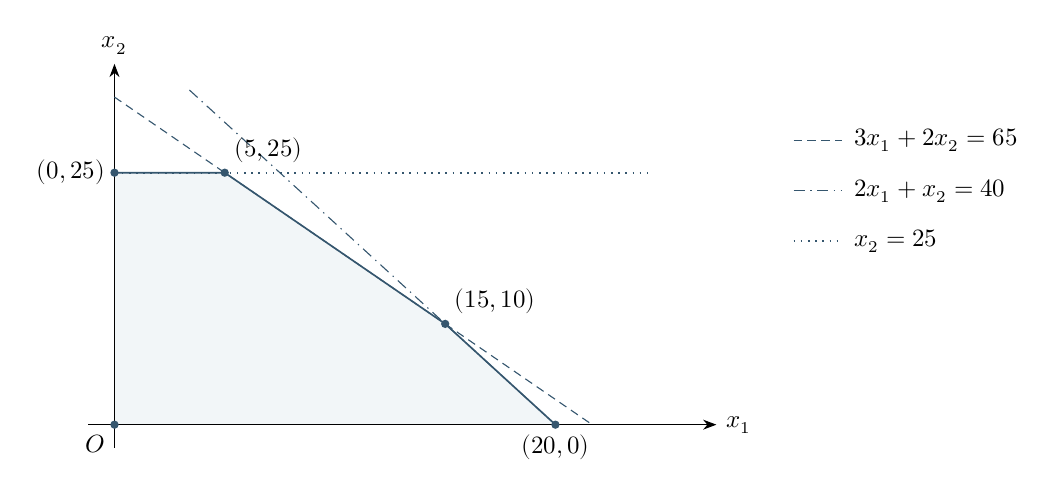
\begin{tikzpicture}[x=0.28cm,y=0.128cm]
\path[region] (0,0)--(20,0)--(15,10)--(5,25)--(0,25)--cycle;
\draw[axis] (-1.2,0)--(27.3,0) node[right] {$x_1$};
\draw[axis] (0,-2.3)--(0,35.8) node[above] {$x_2$};
\draw[helper] (0,32.5)--(21.6667,0);
\draw[Theme,dash pattern=on 4pt off 2pt on 0.5pt off 2pt,thin] (3.4,33.2)--(20,0);
\draw[Theme,dotted,semithick] (0,25)--(24.2,25);
\draw[curve] (0,25)--(5,25)--(15,10)--(20,0);
\fill[Theme] (0,0) circle (1.5pt) (20,0) circle (1.5pt) (15,10) circle (1.5pt)
  (5,25) circle (1.5pt) (0,25) circle (1.5pt);
\node[below left] at (0,0) {$O$};
\node[left] at (0,25) {$(0,25)$};
\node[above right] at (5,25) {$(5,25)$};
\node[above right] at (15,10) {$(15,10)$};
\node[below] at (20,0) {$(20,0)$};
\draw[helper] (30.8,28.2)--(33.0,28.2);
\node[right] at (33.1,28.2) {$3x_1+2x_2=65$};
\draw[Theme,dash pattern=on 4pt off 2pt on 0.5pt off 2pt,thin] (30.8,23.2)--(33.0,23.2);
\node[right] at (33.1,23.2) {$2x_1+x_2=40$};
\draw[Theme,dotted,semithick] (30.8,18.2)--(33.0,18.2);
\node[right] at (33.1,18.2) {$x_2=25$};
\end{tikzpicture}
\diagramcaption{删去三个松弛坐标后，五个极点成为平面可行域的五个顶角}
\end{center}

\subsection{从基矩阵找极方向}
在非空标准形多面体中，先用式 \eqref{eq:recession} 判断一个非零向量是否能一直走。要进一步找\term{极方向}，可在某个基 $B$ 的非基列中挑一列 $a_j$。令相应的 $d_j=1$，其余非基分量为零。由 $Ad=0$ 得
\begin{equation}\label{eq:basicray}
d_B=-B^{-1}a_j,\qquad d_N=e_j^{(N)} ,
\end{equation}
其中 $e_j^{(N)}$ 表示非基坐标中与 $a_j$ 对应的单位向量。若 $B^{-1}a_j\le0$，则式 \eqref{eq:basicray} 给出一条极射线上的代表。此处基矩阵只需可逆，$B^{-1}b\ge0$ 是筛选极点时的条件。

为什么此式找得全？设 $d\in\operatorname{rec}P\setminus\{0\}$，令 $I=\{i:d_i>0\}$。若 $\ker A_I$ 的维数大于 $1$，可在其中取与 $d_I$ 不共线的扰动，延拓成 $I$ 外为零的 $u$。对足够小的 $\varepsilon>0$，$d+\varepsilon u$ 和 $d-\varepsilon u$ 都在衰退锥中，其平均值为 $d$，且不与 $d$ 同向。若 $\ker A_I$ 恰为一维，$d$ 的任何锥内分解在 $I$ 外都为零，两项在 $I$ 上都只能为 $d_I$ 的非负倍数。因此
\[
d\text{ 是极方向}\quad\Longleftrightarrow\quad \rank A_I=|I|-1 .
\]
在极方向的正分量中挑一个 $j$，用正倍数缩放使 $d_j=1$。$\ker A_I$ 的唯一线性关系中，第 $j$ 个系数非零。删去 $a_j$ 后，$I$ 中剩余的列线性无关，且张成空间已包含 $a_j$。扩充为基时可跳过 $a_j$，于是 $d$ 满足式 \eqref{eq:basicray}。反过来，按该式得到的非负向量，其正分量对应列除 $a_j$ 外都属于同一组基，且 $Ad=0$ 给出一条非零关系，所以这些列的秩恰为 $|I|-1$。

每个基至多有 $n-m$ 根非基列可检查。按正倍数视为同一条射线，极射线数至多为 $(n-m)\binom{n}{m}$。在上一例中，$A$ 的各列均非负且没有全零列，因此 $d\ge0$ 且 $Ad=0$ 迫使 $d=0$。该多面体没有非零衰退方向。

\Needspace{11\baselineskip}
\subsection{极点与极方向的表示定理}
\begin{infobox}{定理\quad 非空标准形多面体的表示}
设非空 $P=\{x:Ax=b,\ x\ge0\}$ 的极点为 $v_1,\ldots,v_k$，所有极射线各选一个代表 $r_1,\ldots,r_q$。则每个 $x\in P$ 都可写成
\begin{equation}\label{eq:representation}
 x=\sum_{i=1}^k\lambda_i v_i+\sum_{j=1}^q\mu_j r_j,
 \qquad \lambda_i\ge0,\quad\sum_{i=1}^k\lambda_i=1,\quad\mu_j\ge0 .
\end{equation}
第一个和式是极点的凸组合，第二个是极方向的非负组合。若无极射线，第二个和式取零。满足式 \eqref{eq:representation} 的点也都属于 $P$。
\end{infobox}

\begin{worked}{在无界多面体中拆出极点与极方向}
令 $P=\{x\in\R^3:x_1+x_2-x_3=1,\ x\ge0\}$。求极点及极方向，并对 $x=(2,1,2)\transpose$ 写出一种表示。
\end{worked}
\sol
从三列 $(1),(1),(-1)$ 中选一列作基，分别得到三种基本解 $(1,0,0)\transpose$、$(0,1,0)\transpose$、$(0,0,-1)\transpose$。前两种满足非负性，记作 $v_1,v_2$。衰退方向满足 $d_3=d_1+d_2$，可以写为
\[
d=d_1(1,0,1)\transpose+d_2(0,1,1)\transpose,\qquad d_1,d_2\ge0 .
\]
令 $r_1=(1,0,1)\transpose$、$r_2=(0,1,1)\transpose$。两者各只有一个自由的正分量 $d_1$ 或 $d_2$，因此都是极方向。若 $d_1,d_2$ 同时为正，上式已将它拆成不同方向的两项。于是
\[
x=\tfrac23 v_1+\tfrac13 v_2+\tfrac43 r_1+\tfrac23 r_2
 =(2,1,2)\transpose .
\]
压到 $x_1,x_2$ 平面后，线段 $x_1+x_2=1$ 由两个极点连成。沿水平方向向右或沿竖直方向向上，都可从这条线段一直走。$x_3=x_1+x_2-1$ 随移动增长。

\Needspace{14\baselineskip}
\begin{center}
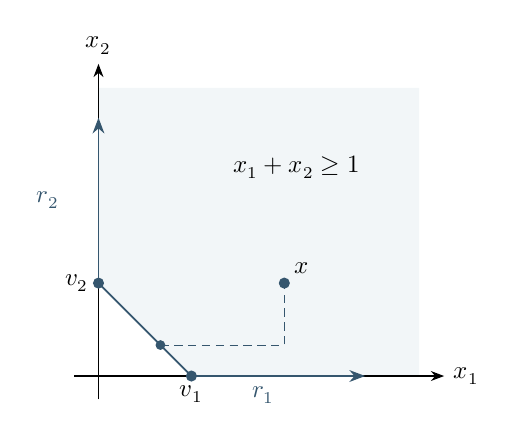
\begin{tikzpicture}[scale=1.18]
\path[region] (0,1)--(1,0)--(3.45,0)--(3.45,3.10)--(0,3.10)--cycle;
\draw[axis] (-0.26,0)--(3.72,0) node[right] {$x_1$};
\draw[axis] (0,-0.25)--(0,3.36) node[above] {$x_2$};
\draw[curve] (0,1)--(1,0);
\draw[Theme,->,semithick] (1,0)--(2.87,0)
 node[midway,below] {$r_1$ 的投影};
\draw[Theme,->,semithick] (0,1)--(0,2.78)
 node[midway,left] {$r_2$ 的投影};
\draw[helper] (0.6667,0.3333)--(2,0.3333)--(2,1);
\fill[Theme] (1,0) circle (1.7pt) (0,1) circle (1.7pt)
 (0.6667,0.3333) circle (1.5pt) (2,1) circle (1.7pt);
\node[below] at (1,0) {$v_1$};
\node[left] at (0,1) {$v_2$};
\node[above right] at (2,1) {$x$};
\node at (2.13,2.25) {$x_1+x_2\ge1$};
\end{tikzpicture}
\diagramcaption{先取极点连线上的点，再沿两条方向移动可到达区域中的点}
\end{center}

\subsubsection*{表示定理的推导}
取任意 $x\in P$。如果它的正分量对应列线性无关，$x$ 已经是极点。否则在这些正分量上选非零扰动 $u$，使 $Au=0$，其余分量为零。
\begin{itemize}
\item 若 $u$ 有正有负，可以沿 $u$ 及 $-u$ 各走到第一个正坐标降为零的位置。记两段步长为 $a,b>0$，所得点 $x^+=x+au$、$x^-=x-bu$ 都可行，正分量也都少于 $x$。点 $x$ 是这两点的凸组合，权重依次为 $b/(a+b)$ 与 $a/(a+b)$。
\item 若 $u$ 的非零分量同号，可翻转符号使 $u\ge0$。取 $b=\min_{u_i>0}x_i/u_i$，则 $x-bu$ 可行且正分量减少。剩余的 $bu$ 是衰退锥中的向量。
\end{itemize}
每次递归都减少参与的正分量数，最终将 $x$ 拆成极点的凸组合及衰退向量的非负组合。要把衰退向量进一步拆成极方向，可将非零 $d\ge0$ 除以其分量和，在切片 $\{d:Ad=0,\ d\ge0,\ \sum_i d_i=1\}$ 中研究。切片中可用的扰动满足分量和为零，所以任何非零扰动必有正有负。按上面第一种方法拆分，有限步后得到切片极点的凸组合。切片极点恰好对应极方向，因为将锥内两项按分量和各自归一化，就会把锥内分解变为切片上的凸组合。乘回分量和即可得到式 \eqref{eq:representation}。

反向代入 $Av_i=b$、$Ar_j=0$，用 $\sum_i\lambda_i=1$ 得 $Ax=b$。所有向量和系数均非负，故 $x\ge0$。这也给出线性目标 $c\transpose x$ 的判断方法。若存在 $c\transpose r_j<0$，沿该极方向可让目标值趋于 $-\infty$。若所有 $c\transpose r_j\ge0$，式 \eqref{eq:representation} 表明任何可行值至少为 $\min_i c\transpose v_i$，选相应极点即可取到最小值。零代价方向可以从最优点出发形成整条最优射线。

\subsection{本章练习}
\begin{enumerate}[label=2.\arabic*.,ref=2.\arabic*,leftmargin=3em]
\item\label{ex:local} 对 $f(x)=(x-1)^2$，分别在 $S=[2,4]$ 与 $S=(2,4]$ 上最小化。判断是否有最优解，并求最小值或下确界。若有最优解，判断它是否严格及其导数是否为零。
\item\label{ex:hull} 将 $\conv\{(0,0),(3,0),(0,4)\}$ 写成不等式集合，判断 $(1,2)$ 与 $(2,3)$ 是否属于它。对可行点写出凸组合系数。
\item\label{ex:cone} 设 $K_1=\{(x,y):x\ge0,\ y\ge0\}$，$K_2=\{(x,0):x\ge0\}\cup\{(0,y):y\ge0\}$，$K_3=\{(x,y):x+y\ge1\}$。分别判断是否为凸集、是否为锥。
\item\label{ex:sublevel} 证明 $g(x)=\max\{(x-1)^2,(x+1)^2\}$ 凸，求 $\{x:g(x)\le4\}$ 及 $g'(0;1)$、$g'(0;-1)$。
\item\label{ex:dir} 设 $f(x)=x_1^2+3x_2^2$，$p=(1,1)\transpose$，$d=(1,-2)\transpose$。求 $f'(p;d)$ 和按单位距离的变化率。在 $x_2\ge1$ 下检验 $d$ 是否可行，并给出一个可行下降方向。
\item\label{ex:hess} 对 $f(x)=x_1^2+2a x_1x_2+x_2^2$，求 $f$ 在 $\R^2$ 上凸和严格凸分别需要的参数范围。解释临界参数时发生了什么。
\item\label{ex:optcond} 在 $x_1\ge1,\ x_2\ge2$ 上最小化 $x_1^2+x_2^2$。说明问题的凸性，用式 \eqref{eq:optcond} 验证最优性，并判断唯一性。
\item\label{ex:degenerate} 对 $P=\{x\ge0:x_1+x_2+x_3=1,\ x_2+x_3=0\}$，列出所有基及其基本解。说明为何不同的基可以对应同一个极点。
\item\label{ex:rays} 设 $P=\{x\ge0:x_1+x_2=2,\ x_2+x_3-x_4=1\}$。求全部极点与极方向，对 $(3/2,1/2,2,3/2)\transpose$ 给出式 \eqref{eq:representation} 的分解。
\item\label{ex:unbounded} 沿用练习 \ref{ex:rays} 的可行集，分别最小化 $x_1+x_3-x_4$ 与 $x_1-x_4$。判断每个问题的最优值是否有限，并在取到最优值时写出全部最优解。
\end{enumerate}

\backsection{主要结论与术语}
\begin{center}
\begin{tabularx}{\linewidth}{l Y}
\toprule
待判断的问题 & 可用结论与前提\\
\midrule
建模与验算 & 先定义变量、单位及取值范围，再写目标和约束。用可行样例检查不等号方向、量纲和参数含义。\\
如何作子空间投影 & $z=p+r$，其中 $p\in L$ 且 $r\perp L$。若 $p=U\alpha$，解 $U\transpose U\alpha=U\transpose z$。\\
怎样近似函数值 & 沿 $h$ 的一阶项是 $\nabla f(x)\transpose h$，二阶项是 $\tfrac12h\transpose\nabla^2 f(x)h$。Taylor 展开中两项均取在同一点 $x$。\\
最优解是否存在 & 非空紧集上的连续函数取到最小值。对开集或无界集，直接检验下确界能否取到。\\
集合是否凸 & 任取两点检查整条线段。闭半空间、仿射方程的解集和任何凸集的交都凸。\\
函数是否凸 & 在开凸集上，可微时用式 \eqref{eq:gradient-bound}。二次连续可微时检查 Hesse 矩阵是否处处半正定。\\
约束下如何证最优 & 凸可行集与凸目标保证局部最优也是全局最优。若目标可微，可用式 \eqref{eq:optcond} 检查指向其他可行点的方向。\\
标准形的极点 & 满行秩时选基 $B$，令 $x_N=0$ 并解 $Bx_B=b$。保留非负的基本解，合并重复点。\\
标准形的极方向 & 先满足 $Ad=0,\ d\ge0$。选基和一根非基列，按式 \eqref{eq:basicray} 生成并保留非负向量。\\
线性目标有无下界 & 对非空标准形，任一极方向上 $c\transpose r<0$ 即向下无界。若所有极方向上均非负，至少一个极点取到最小值。\\
\bottomrule
\end{tabularx}
\end{center}

记号 $x^\star$ 表示一个最优解，$f^\star$ 表示最优值。$f'(x;d)$ 沿 $x+td$ 按参数 $t$ 计量。$H\succeq0$ 表示半正定，$H\succ0$ 表示正定。$\conv$ 生成凸包，$\cone$ 生成包含原点的锥，$\operatorname{rec}P$ 收集衰退方向及零向量。

\subsection*{课件与教材对应}
讲义第 \ref{sec:model} 章依据课程课件《运筹学思想与运筹学建模》，对应教材第 1 章（印刷页 1--19）。讲义第 \ref{sec:theory} 章依据课程课件《基本概念和基本理论》，对应教材第 2 章（印刷页 20--36）。课件的钢厂、背包、二次函数和极点案例用于说明相应方法，数值示例和章末练习按自学需要另行编写。

课程教材为侯福均、吴祈宗编著《运筹学与最优化方法》第 3 版，机械工业出版社，2022 年，ISBN 978-7-111-70295-5。凸集分离及凸函数判别可参阅 S. Boyd 与 L. Vandenberghe 的 \href{https://web.stanford.edu/~boyd/cvxbook/}{\textit{Convex Optimization}} 第 2--4 章。

\backsection{练习参考解答}\label{sec:answers}
\subsection*{第 1 章}
\ans{ex:production}
模型为
\[
\max\, (4x_1+3x_2),\qquad
2x_1+x_2\le10,\quad x_1+x_2\le7,\quad x_1\ge2,\quad x_2\ge0 .
\]
对任何可行方案，
$4x_1+3x_2=(2x_1+x_2)+2(x_1+x_2)\le10+2\cdot7=24$。
令两个资源约束同时取等，解得 $x_1=3,x_2=4$，满足最低产量要求，利润达到上界 $24$。两个约束在上界计算中的权重均为正，取到 $24$ 时它们必须同时取等，所以这个最优方案唯一。

\ans{ex:yield}
若给定的是产出，投入分别为 $6/0.6=10$ 吨和 $8/0.8=10$ 吨，合计比率为 $14/20=70\%$，低于 $71\%$。若给定的是投入，产出之和为 $6\cdot0.6+8\cdot0.8=10$ 吨，总比率为 $10/14=5/7$，约为 $71.43\%$，达到指标。

\ans{ex:choose}
用 $x_i\in\{0,1\}$ 表示选项目 $i$，得到
\[
\max\, (4x_1+7x_2+9x_3),\qquad
2x_1+3x_2+4x_3\le6,\quad x_3\le x_1 .
\]
当 $x_3=1$ 时必须有 $x_1=1$，两者用完预算，总收益为 $13$。当 $x_3=0$ 时，选前两个项目的收益最大，为 $11$。所以应选第 1、3 个项目。

\ans{ex:proj}
令 $p=\alpha(1,1,0)\transpose+\beta(0,1,1)\transpose$。由残差分别与两个向量正交，得
\[
 2\alpha+\beta=3,\qquad \alpha+2\beta=2.
\]
解得 $\alpha=4/3,\ \beta=1/3$。所以 $p=(4/3,5/3,1/3)\transpose$，$r=z-p=(2/3,-2/3,2/3)\transpose$。两个内积均为 $2/3-2/3=0$，最短距离为 $\sqrt{3(2/3)^2}=2/\sqrt{3}$。

\ans{ex:orth}
$L$ 中任意向量写成 $(t,-t,0)\transpose$，$t\in\R$。若 $(a-b)t\le2$ 对所有 $t$ 成立，则 $a=b$，$c$ 可任取。若还对所有 $y\ge0$ 成立，分别取 $y=t e_i$，$t>0$，得 $a,b,c\le0$。合并为 $a=b\le0$、$c\le0$。这些条件也足够，因为它们使 $L$ 上的内积恒为零，并使非负向量上的内积非正。

\ans{ex:quadratic}
将 $Q$ 对称化得 $\tfrac12(Q+Q\transpose)=\begin{pmatrix}2&2\\2&4\end{pmatrix}$。于是 $f=x_1^2+2x_1x_2+2x_2^2$，梯度为 $(2x_1+2x_2,\,2x_1+4x_2)\transpose$。代入 $(1,1)$ 得 $(4,6)\transpose$。Hesse 矩阵即给出的对称化矩阵。

\ans{ex:taylor}
$f(x_0)=2$，$\nabla f(x_0)=(2,3)\transpose$，$\nabla^2 f(x_0)=\begin{pmatrix}2&2\\2&2\end{pmatrix}$。将 $h=(s,t)\transpose$ 代入，
\[
 f(x_0+h)=2+2s+3t+s^2+2st+t^2+s^2t.
\]
最后一项就是精确余项，可直接展开 $(1+s)^2(1+t)+(1+t)^2$ 得到。由于 $|s^2t|\le\norm{h}^3$，所以它是 $o(\norm{h}^2)$。

\Needspace{6\baselineskip}
\subsection*{第 2 章}
\ans{ex:local}
在 $x>1$ 的范围内，$f'(x)=2(x-1)>0$，所以 $f$ 严格递增。在 $[2,4]$ 上，左端点 $x=2$ 是严格全局最优解，最小值为 $1$，且 $f'(2)=2$。这一点只能沿向右的可行方向比较。若去掉左端点，$x\downarrow2$ 时仍可逼近 $1$，但区间内各点值都大于 $1$，故下确界为 $1$ 且没有最优解。

\ans{ex:hull}
若三点的权重为 $\lambda_1,\lambda_2,\lambda_3$，则 $x_1=3\lambda_2$、$x_2=4\lambda_3$。由权重非负且和为 $1$，得到 $x_1,x_2\ge0$、$x_1/3+x_2/4\le1$。反向可令 $\lambda_2=x_1/3,\lambda_3=x_2/4$，再补齐 $\lambda_1$。点 $(1,2)$ 的权重为 $(1/6,1/3,1/2)$，可行。点 $(2,3)$ 有 $2/3+3/4=17/12>1$，在凸包外。

\ans{ex:cone}
$K_1$ 对凸组合及正数缩放都封闭，是凸锥。$K_2$ 中每一点正数缩放后仍在原来的轴上，因此是锥。但 $(1,0),(0,1)$ 的中点 $(1/2,1/2)$ 不在任一轴上，所以它不凸。$K_3$ 是闭半空间，因而凸。由于 $(1,0)\in K_3$ 而其一半 $(1/2,0)$ 在集合外，所以它不满足锥的缩放条件。

\ans{ex:sublevel}
取两个凸平方函数的逐点最大值，所得 $g$ 凸。展开得 $g(x)=(|x|+1)^2$，于是 $g(x)\le4$ 等价于 $|x|\le1$。$t>0$ 时，$g(t)=g(-t)=1+2t+t^2$，所以两个方向的差商都是 $2+t$，右极限均为 $2$。

\ans{ex:dir}
$\nabla f(p)=(2,6)\transpose$，与 $d$ 的内积为 $2-12=-10$。单位距离的变化率为 $-10/\sqrt5=-2\sqrt5$。$p+td$ 的第二分量为 $1-2t$，对 $t>0$ 立即违反约束。取 $\tilde d=(-1,0)\transpose$ 可保持第二分量为 $1$，方向导数为 $-2$。

\ans{ex:hess}
Hesse 矩阵为 $\begin{pmatrix}2&2a\\2a&2\end{pmatrix}$，特征值为 $2(1+a)$ 与 $2(1-a)$。因此凸性的充要条件是 $|a|\le1$。$|a|<1$ 时矩阵正定，函数严格凸。$a=1$ 或 $a=-1$ 时，函数分别为 $(x_1+x_2)^2$ 或 $(x_1-x_2)^2$，存在一整条函数值为零的直线，所以不严格凸。

\ans{ex:optcond}
可行集是闭半空间的交，目标 Hesse 矩阵为 $2I$，故严格凸。取 $x^\star=(1,2)\transpose$，对每个可行 $y$，有 $\nabla f(x^\star)\transpose(y-x^\star)=2(y_1-1)+4(y_2-2)\ge0$。由式 \eqref{eq:optcond} 得 $x^\star$ 全局最优，最优值为 $5$，且严格凸性给出唯一性。

\ans{ex:degenerate}
约束矩阵的第 2、3 列相同，基只能取 $(1,2)$ 或 $(1,3)$。由 $x_2+x_3=0$ 和非负性知 $x_2=x_3=0$，再由第一条等式得 $x_1=1$。两个基本解都是 $(1,0,0)\transpose$，且各有一个基变量为零，故同一个退化极点对应两组基。

\ans{ex:rays}
两行约束使矩阵满行秩。可行的两列基为 $(1,2),(1,3),(2,4)$，分别给出
\[
v_1=(1,1,0,0)\transpose,\qquad v_2=(2,0,1,0)\transpose,\qquad
v_3=(0,2,0,1)\transpose.
\]
候选 $(3,4)$ 奇异，$(1,4)$ 与 $(2,3)$ 分别产生负的 $x_4$、$x_3$。由 $Ad=0$、$d\ge0$ 得 $d_1=d_2=0$、$d_3=d_4\ge0$，故唯一极射线可取 $r=(0,0,1,1)\transpose$。题给点为 $\tfrac12v_1+\tfrac12v_2+\tfrac32r$。

\ans{ex:unbounded}
第一目标在 $r$ 上的代价为零。在三个极点上的值依次为 $1,3,-1$，最小值为 $-1$。由等式直接化简，$x_1+x_3-x_4=2x_1-1$，恰在 $x_1=0$ 时取到 $-1$。所以全部最优解为 $(0,2,t,1+t)\transpose$，$t\ge0$。第二目标在 $r$ 上的代价为 $-1$，沿 $v_3+tr$ 得 $x_1-x_4=-1-t\to-\infty$，故向下无界。

\end{document}
